\documentclass[12pt]{article}
\usepackage{graphicx}
\usepackage[portuguese]{babel}
\usepackage[utf8]{inputenc}
\usepackage[T1]{fontenc}
\begin{document}
\begin{titlepage}
\begin{center}
\begin{figure}[htp]
\begin{center}

\includegraphics[scale=1.5]{image.jpg}
\end{center}
\end{figure}
\begin{huge}
Trabalho de Base de Dados\\
\end{huge}
Rúben Peixoto nº37514\\
Sarah Simon nº38116\\
\end{center}
\end{titlepage}
\begin{titlepage}
\section*{\underline{Enunciado}}
\begin{center}
\begin{LARGE}
Florista
\end{LARGE}
\end{center}
Uma empresa pretende inserir uma base de dados para não só gerir os stocks do armazém como também gerir o pagamento dos salários dos seus funcionários.

A empresa vende vários artigos ligados a floricultura. Sempre que se queira a empresa deve saber a quantidade de artigos existente no armazém. O cliente ao ir à loja tem a opção de comprar os artigos presentes na loja ou,  se o mesmo quiser algo diferenciado, pode optar por fazer uma encomenda para o funcionário orientado para essa função. O cliente é identificado pelo número de cliente e pelo NIF. Tanto para a compra do artigo sem encomenda como para a compra com encomenda é necessário um código que os identifique assim como o valor pago. Para além do mais, as encomendas são pedidas e entregues no mesmo dia.
Para a compra temos o número de funcionário, o número do artigo, numero do cliente, número de compra, tipo de compra.

Os artigos vão ser encontrados num armazém denominado “Stocks”. Nele vai nos ser informado o nome do produto, quantidade, número do artigo, número do fornecedor. Esta empresa é de pequena dimensão, logo, teremos 2 funcionários. Temos um funcionário para a reposição e outro para a caixa. Todos os funcionários são identificados pelo NIF, nome, morada, BI, salário.

O funcionário que trabalha na reposição recebe todos os dias artigos de vários fornecedores. Esse fornecedor é identificado pelo nome, número do fornecedor e número de encomenda.

O cliente é identificado com o número do cliente, número de identificação fiscal e o número da compra.\\
Legenda:

numA = número do artigo

numF = número do funcionário

numC = número do cliente

tipoCompra = tipo de compra (compra direta ou encomenda)

numFornecedor = número do fornecedor

nomef = nome do forncedor

nomeP = nome do produto
\end{titlepage}
\begin{titlepage}
\section*{\underline{Modelo Entidade}}
\begin{figure}[h]
\begin{center}
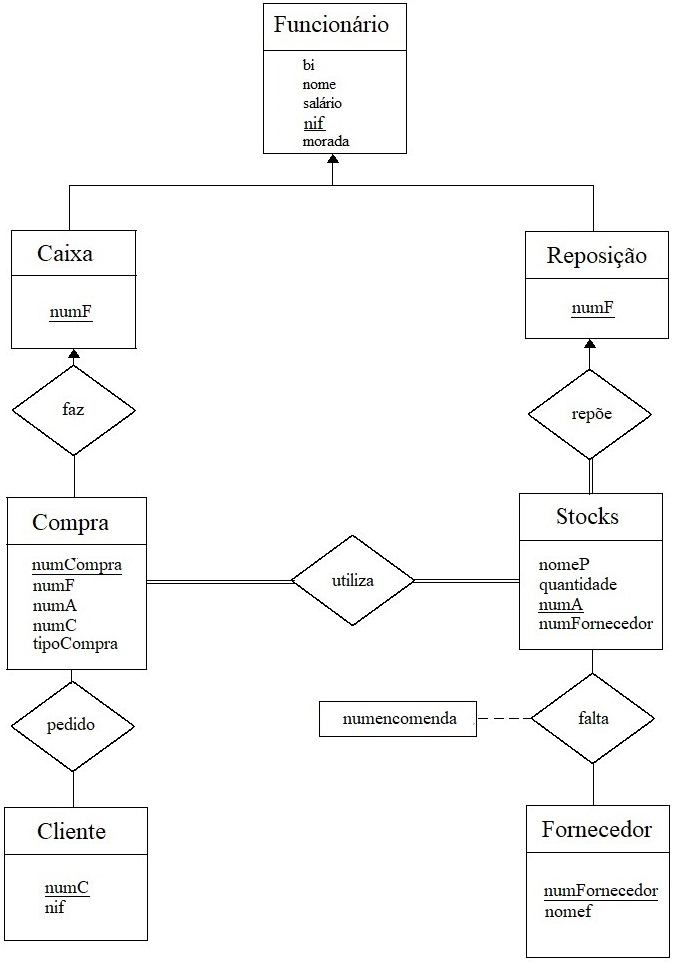
\includegraphics[scale=0.845]{ModeloBD.jpg}
\end{center}
\end{figure}
\end{titlepage}
\begin{titlepage}
\section*{\underline{Modelo Relacional}}
funcionario = (\underline{nif}, bi ,nome, morada, salário)\\
cliente     = (\underline{numC}, nif)\\
compra      = (numA, numF, numC, tipoCompra, \underline{numCompra})\\
fornecedor  = (\underline{numFornecedor}, nomef)\\
stocks      = (nomeP, quantidade, \underline{numA}, numFornecedor)\\
caixa       = (\underline{numF})\\
reposição   = (\underline{numF})\\
repõe       = (\underline{numF}, \underline{numA})\\
faz         = (\underline{numF}, \underline{numCompra})\\
utiliza     = (\underline{numCompra}, \underline{numA})\\
pedido      = (\underline{numCompra}, \underline{numC})\\
falta       = (numencomenda, \underline{numFornecedor}, \underline{numA})
\section*{\underline{Dependências Funcionais}}
numC $\longrightarrow$ nif\\
numF $\longrightarrow$ numA, numCompra\\
numFornecedor $\longrightarrow$ nomef\\
nomeP $\longrightarrow$ quantidade\\
numCompra, numC $\longrightarrow$ tipoCompra\\ 
numA $\longrightarrow$ numFornecedor,nomeP\\
numCompra $\longrightarrow$ numF, numC, tipoCompra
\section*{\underline{Correção das dependências funcionais}}
	A dependência funcional "nomeP $\longrightarrow$ quantidade" não está na 3 forma normal uma que existe colunas não chave a depender de outra coluna não chave.\\
Para corrigir esta situação podermos juntar "nomeP $\longrightarrow$ quantidade" com "numA $\longrightarrow$ numFornecedor,nomeP" ficando:
\begin{center}
numA $\longrightarrow$ numFornecedor, nomeP, quantidade
\end{center}
\end{titlepage}
\begin{titlepage}
A dependência funcional "numCompra $\longrightarrow$ numF, numC, tipoCompra"  não está em Boyce-Codd forma normal porque nem todos os atributos não chave dependem diretamente da chave primária, isto é, não há dependências entre atributos não chave. Então desmonta-se esta dependência em duas:
\begin{center}
r1 = (numCompra, numF, numC, tipoCompra)\\
r2 = (tipoCompra, numCompra)
\end{center}
\end{titlepage}
\end{document}